% Drawing 74/06-3 -- folder 74, batch 06, archive page 105 (PDF page 106).
% Transcription: en tête de page : une étoile de triangles (deux sommets épais reliés, portant chacun plusieurs triangles), marquée $\sigma_{t_0}$ ; un signe en gras ; deux triangles opposés par un sommet ; un triangle isolé
% Kind: star of triangles, opposed triangles. Method 2 (schematic redraw from the facsimile). Status: ok.
% Notes: Three junctions: the two thick vertices (upper and lower) joined by a heavy stroke, and a third junction at the left joined to both. Thin triangles, each with its two long sides starting at its junction and closed by a short stroke at the far end: three from the left junction, three from the upper thick vertex (the first in heavy ink, ending in a blot), three from the lower one. A short tick crosses the stroke from the left junction to the upper vertex, and a short stroke stands beside the heavy stroke below the upper vertex. sigma_{t_0}; a bold sign drawn as it stands (a loop open at the upper right with a bar into its centre, its reading unsure); two triangles opposed at a vertex (the upper one bold); an isolated triangle. Nothing is struck. Overlay check 2026-11-13 (issue 147, Claude claude-opus-5-5): the redraw, rasterised by the skill's previewer (not compiled: no TeX in the session), laid over the 300 dpi colour crop of the scan (261 ppi). The earlier redraw lay 1 to 3 units off its ink (the lower thick vertex 1.5 units to the left, the wedges of the upper and lower vertices and the two opposed triangles at the right 1 to 3 units off) and lacked the two short strokes: every triangle redrawn through its tips read on the scan, the two opposed triangles moved onto their ink (the isolated triangle already lay on its own), the loop enlarged to its size on the page, and the two short strokes added. Matches the facsimile.
% Coordinates: 1 unit = 1 mm = 1/100 of the crop width (bbox in page fractions: [0.08, 0.08, 0.85, 0.3]).
% Redrawn by Claude (claude-opus-5-5), issue #73, 2026-11-09; not checked by a human; not compiled (no TeX in the session).
% Checked by Claude (claude-opus-5-5) 2026-11-13 (issue #147): overlaid on the 300 dpi colour facsimile and corrected; not compiled (no TeX in the session). Status: ok.
% Rights: reproduces part of the work -- behind RENDER_TRANSCRIPTS, never published by itself.
\documentclass[tikz,border=3pt]{standalone}
\usepackage{amsmath,amssymb}
\usetikzlibrary{patterns,arrows.meta}
\tikzset{pencil/.style={black!45}, struck/.style={black!35}, mark/.style={circle,draw,inner sep=1.3pt}, pt/.style={circle,fill,inner sep=0.9pt}, opt/.style={circle,draw,fill=white,inner sep=1.1pt}}
\begin{document}
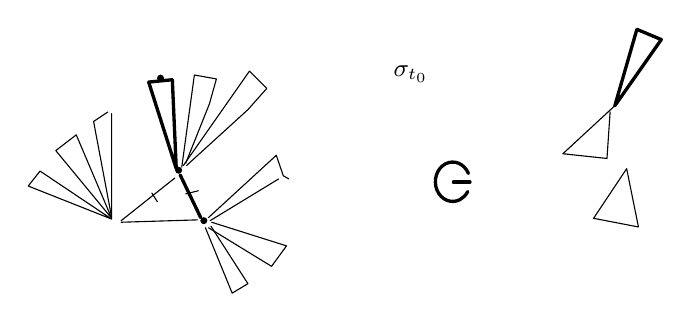
\begin{tikzpicture}[x=1mm,y=1mm,line cap=round,line join=round,font=\scriptsize]
\draw (16.5,-29.8) -- (26.2,-29.5);
\draw (16.5,-29.6) -- (23.3,-24.2);
\draw (20.4,-26.1) -- (21.1,-27.2);
\draw (24.7,-26.2) -- (26.3,-25.8);
\draw[very thick] (24,-23.8) -- (26.6,-29.2);
\draw (4.7,-25.2) -- (15.3,-29.4) -- (6.2,-23.3) -- (4.7,-25.2);
\draw (8.2,-20.7) -- (15.3,-29.3) -- (10.8,-18.7) -- (8.2,-20.7);
\draw (13,-17) -- (15.3,-29.2) -- (15.3,-16);
\draw (13,-17) -- (14.8,-15.8);
\draw[very thick] (20,-12) -- (23.5,-23) -- (23,-11.7);
\draw[very thick] (20,-12) -- (23,-11.7);
\node[pt] at (21.5,-11.5) {};
\draw (24.2,-22.8) -- (25.8,-11.1) -- (28.6,-11.6) -- (27.7,-14.8) -- (24.7,-22.3);
\draw (24.4,-22.6) -- (32.8,-10.6) -- (35,-12.8) -- (32.6,-15.5) -- (24.8,-22.6);
\draw (27.6,-29.2) -- (36.2,-21.3);
\draw (27.8,-29.6) -- (36.5,-24.3);
\draw (36.2,-21.3) -- (37.1,-23.9) -- (37.8,-24.3);
\draw (28,-29.8) -- (37.5,-32.8) -- (35.6,-35.4) -- (27.6,-30.5);
\draw (27.9,-30.3) -- (32.6,-37.6) -- (30.6,-38.8) -- (27.2,-30.5);
\node[pt] at (23.8,-23.2) {};
\node[pt] at (27,-29.6) {};
\node[inner sep=1pt] at (53.3,-11) {\small $\sigma_{t_0}$};
\draw[very thick] (60.6,-23.6) arc[start angle=25, end angle=330, x radius=2.2, y radius=2.5];
\draw[very thick] (58.7,-24.7) -- (60.8,-24.7);
\draw[very thick] (82,-5.3) -- (85.1,-6.6) -- (79.2,-15) -- (82,-5.3);
\draw (79.2,-15) -- (72.6,-21.1) -- (78.2,-21.7) -- (78.6,-15.8);
\draw (80.7,-23) -- (76.5,-29.3) -- (82.2,-30.4) -- (80.7,-23);
\end{tikzpicture}
\end{document}
